\documentclass{beamer}
\usepackage[T1]{fontenc}
\usepackage[english]{babel}
\usepackage{lmodern}
\usepackage{amsmath,amssymb}
\usepackage{algorithm}
\usepackage{algorithmic}
\usepackage{graphicx}
\usepackage{subcaption}
\usepackage{caption}
\usepackage{tikz}
\usetikzlibrary{shapes.geometric,positioning,calc,fit}
\usetikzlibrary{overlay-beamer-styles}
\usepackage{booktabs,multicol,stackengine}
\usepackage[table,dvipsnames]{xcolor}
\usepackage{cancel}
\usepackage{moresize}
\usepackage{hyperref}

\usepackage{listings}
\definecolor{nus-orange}{RGB}{239,124,0}
\definecolor{nus-blue}{RGB}{0,61,124}
\definecolor{halfgray}{gray}{0.55}

\lstset{
  basicstyle=\ttfamily\scriptsize,
  keywordstyle=\bfseries\color{nus-blue},
  stringstyle=\color{ForestGreen},
  numbers=left,
  numberstyle=\scriptsize\color{halfgray},
  rulesepcolor=\color{nus-orange},
  frame=shadowbox,
  columns=flexible,
  showstringspaces=false,
  keepspaces=true,
  tabsize=2,
  breaklines=true
}

\renewcommand{\figurename}{Figure}
\renewcommand{\algorithmname}{Algorithm}

\usepackage{SHU}
\setbeamersize{text margin left=7mm, text margin right=7mm}
% VITAL STUFF
\renewcommand\epsilon\varepsilon
\renewcommand\phi\varphi
\renewcommand\leq\leqslant
\renewcommand\geq\geqslant
\newcommand\defeq{\stackrel{\mathrm{def}}{=}}

% For revision
\newcommand\rev[1]{{#1}}

% COMMENTS
\newcommand\mikael[1]{\textcolor{orange}{[\textbf{Mikaël:} #1]}}
\newcommand\pierre[1]{\textcolor{magenta}{[\textbf{Pierre:} #1]}}
\newcommand\pratik[1]{\textcolor{blue}{[\textbf{Pratik:} #1]}}

% SMOL SYMBOLS
\newcommand\calF{\mathcal{F}}
\newcommand\RR{\mathbb{R}}
\newcommand\QQ{\mathbb{Q}}
\newcommand\bD{\mathbf{D}}

% REDUCTIONS
\newcommand{\tr}{\leq_{\mathsf{P}}}
\newcommand{\equivt}{\equiv_{\mathsf{P}}}

% PROBLEMS
\newcommand\escore{\mathsf{EScore}}
\newcommand\score{\mathsf{Score}}
\newcommand\eshapley{\escore_{\cshapley}}
\newcommand\shapley{\score_{\cshapley}}
\newcommand\ebanzhaf{\escore_{\cbanzhaf}}
\newcommand\banzhaf{\score_{\cbanzhaf}}
\newcommand\ev{\mathsf{EV}}
\newcommand\evs{\mathsf{EV}_\star}
\newcommand\ennv{\mathsf{ENV}} % \env was already defined
\newcommand\envss{\mathsf{ENV}_{\star,\star}}
\newcommand\mc{\mathsf{MC}}
\newcommand\env{\mathsf{ENV}}

% NOTATIONS
\newcommand\vars{\mathsf{Vars}}
\newcommand\out{\mathsf{out}} % for output gate
\newcommand\cshapley{c_{\mathrm{Shapley}}}
\newcommand\cbanzhaf{c_{\mathrm{Banzhaf}}}
\newcommand\ar{\mathsf{ar}}
\newcommand\const{\mathsf{Const}}
\newcommand{\pqe}{\mathrm{PQE}}
\newcommand\prov{\mathrm{Prov}}

% For algorithm2e
\newcommand{\hrulealg}[0]{\vspace{1mm} \hrule \vspace{1mm}}

% For alignment of numbers
\newcommand{\0}{\phantom{0}}

% Example
\newcommand{\phiex}{\phi_{\mathrm{ex}}}


% Functional dependency helpers
\newcommand\fd[2]{\{#1\} \rightarrow \{#2\}}
\newcommand\cl[1]{\{#1\}^+}
\newcommand\Cstar{C^{*}}

\title{IT5008: Tutorial 8 --- Functional Dependencies}
\author{\href{https://pratik2358.github.io/}{Pratik Karmakar}}
\institute{School of Computing,\\ National University of Singapore}
\date{AY26/27 S1}

\begin{document}

\begin{frame}
  \titlepage
  \IfFileExists{nus-logo.png}{
    \begin{figure}[htpb]\centering
      
\includegraphics[keepaspectratio, scale=0.18]{nus-logo.png}
    \end{figure}
  }{}
\end{frame}

%=====================================================================
\section{Example}

\begin{frame}{Example}
\small
\begin{center}
    Example Relation,  $R = \{A,B,C\} \text{ and } \Sigma =\{\{A\} \rightarrow \{B\}, \{B\} \rightarrow \{C\}\}$
\end{center}
\tiny
The column in \alert{red} decides the color of the row: \textcolor{blue}{The rows having same values in the \alert{red} column, have same color}.\\
\textbf{Task:} Check which other columns are following \textcolor{blue}{``same value if same color"} for each deciding (\alert{red}) column. The columns for which this holds, are implied by the \alert{red} column.
\footnotesize
\begin{columns}
    \begin{column}{0.32\textwidth}
        \begin{table}[t]
\centering
\begin{tabular}{ccc}
\toprule
\textbf{\alert{A}} & \textbf{B} & \textbf{C} \\
\toprule
\rowcolor{Dandelion}
a1 & b1 & c1 \\
\rowcolor{Dandelion}
a1 & b1 & c1 \\
\rowcolor{lightgray}
a2 & b2 & c2 \\
\rowcolor{lightgray}
a2 & b2 & c2 \\
\rowcolor{Thistle}
a3 & b3 & c2 \\
\rowcolor{Thistle}
a3 & b3 & c2 \\
\rowcolor{YellowGreen}
a4 & b1 & c1 \\
\rowcolor{YellowGreen}
a4 & b1 & c1 \\
a5 & b2 & c2 \\
\bottomrule
\end{tabular}\\
\pause
$\{\alert{A}\} \rightarrow \{A,B,C\}$
\end{table}
    \end{column}
    \pause
    \begin{column}{0.32\textwidth}
        \begin{table}[t]
\centering
\begin{tabular}{ccc}
\toprule
\textbf{A} & \textbf{\alert{B}} & \textbf{C} \\
\toprule
\rowcolor{Dandelion}
a1 & b1 & c1 \\
\rowcolor{Dandelion}
a1 & b1 & c1 \\
\rowcolor{lightgray}
a2 & b2 & c2 \\
\rowcolor{lightgray}
a2 & b2 & c2 \\
\rowcolor{Thistle}
a3 & b3 & c2 \\
\rowcolor{Thistle}
a3 & b3 & c2 \\
\rowcolor{Dandelion}
a4 & b1 & c1 \\
\rowcolor{Dandelion}
a4 & b1 & c1 \\
\rowcolor{lightgray}
a5 & b2 & c2 \\
\bottomrule
\end{tabular}\\
\pause
$\{\alert{B}\} \rightarrow \{B,C\}$
\end{table}
    \end{column}
    \pause
    \begin{column}{0.32\textwidth}
        \begin{table}[t]
\centering
\begin{tabular}{ccc}
\toprule
\textbf{A} & \textbf{B} & \textbf{\alert{C}} \\
\toprule
\rowcolor{Dandelion}
a1 & b1 & c1 \\
\rowcolor{Dandelion}
a1 & b1 & c1 \\
\rowcolor{lightgray}
a2 & b2 & c2 \\
\rowcolor{lightgray}
a2 & b2 & c2 \\
\rowcolor{lightgray}
a3 & b3 & c2 \\
\rowcolor{lightgray}
a3 & b3 & c2 \\
\rowcolor{Dandelion}
a4 & b1 & c1 \\
\rowcolor{Dandelion}
a4 & b1 & c1 \\
\rowcolor{lightgray}
a5 & b2 & c2 \\
\bottomrule
\end{tabular}\\
\pause
$\{\alert{C}\} \rightarrow \{C\}$
\end{table}
    \end{column}
\end{columns}
\end{frame}

%=====================================================================
\section{Questions}

\begin{frame}{Scenario}
\small
Your company, \emph{Apasaja Private Limited}, is commissioned by an online company offering several services to design the relational schema for the management of their users' profiles. A service is fully described and identified by its name. Each user can register to one or more services. A user is uniquely identified by her email as well as by her mobile number. Each user has both a postal address and a country of residence. The postal address, however, unambiguously identifies the country in which it is located. There can be several users with the same address.
\medskip

We are given the following abstract schema for this application.
\begin{itemize}
  \item $R = \{A, B, C, D, E\}$
  \item $\Sigma = \{\, \fd{A}{A,B,C},\ \fd{A,B}{A},\ \fd{B,C}{A,D},\ \fd{B}{A,B},\ \fd{C}{D} \,\}$
\end{itemize}
\end{frame}

\begin{frame}{Questions}
\footnotesize
\textbf{Preliminary} \textit{(not discussed in class)}
\begin{enumerate}
  \item[\textbf{1.}] \textbf{Schema.}
  \begin{enumerate}
    \item[(a)] Draw the entity-relationship diagram.
    \item[(b)] Translate the entity-relationship diagram into a schema.
    \item[(c)] From $\Sigma$, the text, the ER diagram and the schema, figure out the mapping of the attributes and the letters.
  \end{enumerate}
\end{enumerate}
\medskip
\textbf{Discussion}
\begin{enumerate}
  \item[\textbf{2.}] \textbf{Calculations.}
  \begin{enumerate}
    \item[(a)] Compute the attribute closures of the subsets of attributes of $R$ with $\Sigma$ in order to find the candidate keys of $R$ with $\Sigma$.
    \item[(b)] Find the prime attributes of $R$ with $\Sigma$.
  \end{enumerate}
  \item[\textbf{3.}] \textbf{Basis or Cover.}
  \begin{enumerate}
    \item[(a)] Compute one possible minimal cover (a.k.a.\ minimal basis) of $R$ with $\Sigma$.
    \item[(b)] Compute one possible canonical cover of $R$ with $\Sigma$.
  \end{enumerate}
\end{enumerate}
\end{frame}

%=====================================================================
\section{Preliminary}

\begin{frame}{1(a). Entity-Relationship Diagram}
\begin{center}
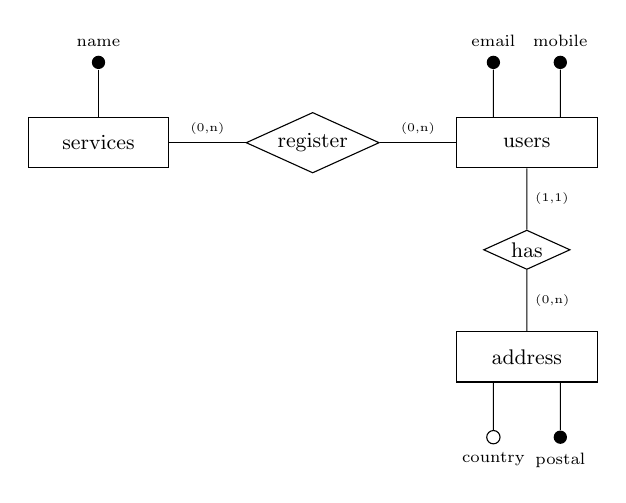
\begin{tikzpicture}[scale=0.85, every node/.style={transform shape},
    ent/.style={draw, minimum width=2.1cm, minimum height=0.75cm, font=\small},
    rel/.style={draw, diamond, aspect=2.2, inner sep=1.5pt, font=\small},
    key/.style={circle, fill=black, inner sep=2pt},
    att/.style={circle, draw, fill=white, inner sep=2pt},
    lbl/.style={font=\scriptsize},
    card/.style={font=\tiny}
  ]
  \node[ent] (services) at (0,0) {services};
  \node[rel] (register) at (3.2,0) {register};
  \node[ent] (users) at (6.4,0) {users};
  \node[rel] (has) at (6.4,-1.6) {has};
  \node[ent] (address) at (6.4,-3.2) {address};

  \draw (services) -- node[card, above] {(0,n)} (register);
  \draw (register) -- node[card, above] {(0,n)} (users);
  \draw (users) -- node[card, right] {(1,1)} (has);
  \draw (has) -- node[card, right] {(0,n)} (address);

  % attributes: filled = key
  \node[key] (sname) at (0,1.2) {};
  \node[lbl, above] at (sname.north) {name};
  \draw (sname) -- (services);

  \node[key] (email) at (5.9,1.2) {};
  \node[lbl, above] at (email.north) {email};
  \draw (email) -- (email |- users.north);
  \node[key] (mobile) at (6.9,1.2) {};
  \node[lbl, above] at (mobile.north) {mobile};
  \draw (mobile) -- (mobile |- users.north);

  \node[att] (country) at (5.9,-4.4) {};
  \node[lbl, below] at (country.south) {country};
  \draw (country) -- (country |- address.south);
  \node[key] (postal) at (6.9,-4.4) {};
  \node[lbl, below] at (postal.south) {postal};
  \draw (postal) -- (postal |- address.south);
\end{tikzpicture}
\end{center}
\scriptsize
\textbf{Filled} circles are keys: \texttt{email} and \texttt{mobile} each identify a user; \texttt{postal} identifies an address (and so its \texttt{country}).
\end{frame}

\begin{frame}[fragile]{1(b). Translating to a Schema}
\footnotesize
One possible answer:
\begin{columns}[t,onlytextwidth]
\column{0.45\textwidth}
\begin{lstlisting}[language=SQL,numbers=none]
CREATE TABLE services (
  name VARCHAR(256) PRIMARY KEY
);

CREATE TABLE address (
  postal VARCHAR(10) PRIMARY KEY,
  country VARCHAR(100) NOT NULL
);
\end{lstlisting}
\column{0.05\textwidth}
\column{0.45\textwidth}
\begin{lstlisting}[language=SQL,numbers=none]
CREATE TABLE users (
  email VARCHAR(100) PRIMARY KEY,
  mobile NUMERIC UNIQUE NOT NULL,
  postal VARCHAR(10)
    REFERENCES address(postal)
);

CREATE TABLE register (
  name VARCHAR(256)
    REFERENCES services(name),
  email VARCHAR(100)
    REFERENCES users(email),
  PRIMARY KEY (name, email)
);
\end{lstlisting}
\end{columns}
\medskip
\begin{itemize}
  \item \texttt{has} is $(1,1)$ on the \texttt{users} side, so it folds into \texttt{users} as a foreign key.
  \item \texttt{mobile} is a second key: \texttt{UNIQUE NOT NULL}.
\end{itemize}
\end{frame}

\begin{frame}{1(c). Mapping Attributes to Letters}
\footnotesize
Your company, Apasaja Private Limited, is commissioned by an online company offering several services to design the relational schema for the management of their users' profiles. \textcolor{red}{A service is fully described and identified by its name}. Each user can register to one or more services. \textcolor{blue}{A user is uniquely identified by her \textbf{email} as well as by her \textbf{mobile number}}. Each user has both a postal address and a country of residence. \textcolor{teal}{The \textbf{postal address}, however, unambiguously identifies the \textbf{country} in which it is located}. There can be several users with the same address.
\medskip

\normalsize
\pause
\textcolor{blue}{$\fd{A}{A,B,C} \implies \fd{A}{B}$ and $\fd{B}{A}$: $A$ and $B$ are email and mobile number, or vice versa.}
\medskip

\pause
\textcolor{teal}{$\fd{C}{D}$: $C$ is the postal address and $D$ is the country.}
\medskip

\pause
\textcolor{red}{The service name neither depends on anything nor implies anything. Thus $E$ is the service name.}
\end{frame}

\begin{frame}{1(c). The Mapping}
\begin{center}
\renewcommand{\arraystretch}{1.3}
\begin{tabular}{ll}
\toprule
\textbf{Attribute} & \textbf{Letter} \\
\midrule
\texttt{email} / \texttt{mobile} & $A$ / $B$ (or vice versa) \\
\texttt{postal} & $C$ \\
\texttt{country} & $D$ \\
\texttt{name} (of service) & $E$ \\
\bottomrule
\end{tabular}
\end{center}
\medskip
\small
$R = \{A,B,C,D,E\}$ is one big relation: (\emph{email, mobile, postal, country, service}) --- one row per user \emph{per service} they registered to.
\end{frame}

%=====================================================================
\section{Discussion}

\begin{frame}{2(a). Finding the Candidate Keys}
\footnotesize
\textbf{Observation:} $E$ does not appear on the right-hand side of \emph{any} functional dependency in $\Sigma$. So nothing can derive $E$: it must be in \textbf{every} candidate key.
\medskip

We only need closures of supersets of $\{E\}$:
\begin{itemize}\itemsep1pt
  \pause
  \item \textbf{Cardinality 1}
  \begin{itemize}
    \item $\cl{E} = \{E\}$ \hfill (not a key)
  \end{itemize}
  \pause
  \item \textbf{Cardinality 2}
  \begin{itemize}
    \item $\cl{A,E} = \{A,B,C,D,E\}$ \hfill \alert{(a candidate key)}
    \item $\cl{B,E} = \{A,B,C,D,E\}$ \hfill \alert{(a candidate key)}
    \item $\cl{C,E} = \{C,D,E\}$ \hfill (not a key)
    \item $\cl{D,E} = \{D,E\}$ \hfill (not a key)
  \end{itemize}
  \pause
  \item \textbf{Cardinality 3}, superset of $\{E\}$, but \underline{not a superset of a known candidate key}
  \begin{itemize}
    \item $\cl{C,D,E} = \{C,D,E\}$ \hfill (not a key)
  \end{itemize}
  \pause
  \item Every other set either lacks $E$, or contains $\{A,E\}$ or $\{B,E\}$ (so it is a superkey but not minimal).
\end{itemize}
\pause
\textbf{Candidate keys:} $\alert{\{A,E\}}$ and $\alert{\{B,E\}}$.
\end{frame}

\begin{frame}{2(a). Sanity Check: All 31 Closures}
\scriptsize
Computing every closure by hand is tedious --- the shortcut above saves most of the work. For reference, superkeys in \alert{red}; candidate keys \underline{underlined}.
\medskip

\begin{columns}[t,onlytextwidth]
\tiny
\column{0.33\textwidth}
$\{A\}^+ = \{A,B,C,D\}$\\
$\{B\}^+ = \{A,B,C,D\}$\\
$\{C\}^+ = \{C,D\}$\\
$\{D\}^+ = \{D\}$\\
$\{E\}^+ = \{E\}$\\
$\{A,B\}^+ = \{A,B,C,D\}$\\
$\{A,C\}^+ = \{A,B,C,D\}$\\
$\{A,D\}^+ = \{A,B,C,D\}$\\
$\textcolor{red}{\underline{\{A,E\}^+ = \{A,B,C,D,E\}}}$\\
$\{B,C\}^+ = \{A,B,C,D\}$\\
$\{B,D\}^+ = \{A,B,C,D\}$
\column{0.33\textwidth}
$\textcolor{red}{\underline{\{B,E\}^+ = \{A,B,C,D,E\}}}$\\
$\{C,D\}^+ = \{C,D\}$\\
$\{C,E\}^+ = \{C,D,E\}$\\
$\{D,E\}^+ = \{D,E\}$\\
$\{A,B,C\}^+ = \{A,B,C,D\}$\\
$\{A,B,D\}^+ = \{A,B,C,D\}$\\
$\textcolor{red}{\{A,B,E\}^+ = \{A,B,C,D,E\}}$\\
$\{A,C,D\}^+ = \{A,B,C,D\}$\\
$\textcolor{red}{\{A,C,E\}^+ = \{A,B,C,D,E\}}$\\
$\textcolor{red}{\{A,D,E\}^+ = \{A,B,C,D,E\}}$
\column{0.33\textwidth}
$\{B,C,D\}^+ = \{A,B,C,D\}$\\
$\textcolor{red}{\{B,C,E\}^+ = \{A,B,C,D,E\}}$\\
$\textcolor{red}{\{B,D,E\}^+ = \{A,B,C,D,E\}}$\\
$\{C,D,E\}^+ = \{C,D,E\}$\\
$\{A,B,C,D\}^+ = \{A,B,C,D\}$\\
$\textcolor{red}{\{A,B,C,E\}^+ = \{A,B,C,D,E\}}$\\
$\textcolor{red}{\{A,B,D,E\}^+ = \{A,B,C,D,E\}}$\\
$\textcolor{red}{\{A,C,D,E\}^+ = \{A,B,C,D,E\}}$\\
$\textcolor{red}{\{B,C,D,E\}^+ = \{A,B,C,D,E\}}$\\
$\textcolor{red}{\{A,B,C,D,E\}^+ = \{A,B,C,D,E\}}$
\end{columns}
\medskip
Every red set contains $E$ --- as predicted.
\medskip

\footnotesize
\textbf{Here's some help:} compute closures yourself at \href{https://functionaldepcheckeronline.streamlit.app/}{\textcolor{blue}{\underline{functionaldepcheckeronline.streamlit.app}}}
\end{frame}

\begin{frame}{2(b). Prime Attributes}
\vfill
We have $\alert{\{A,E\}}$ and $\alert{\{B,E\}}$ as the \alert{candidate keys}.
\bigskip

\pause
The attributes participating in the candidate keys are called the \alert{prime attributes}.
\bigskip

\pause
Here the prime attributes are $\alert{\{A, B, E\}}$ --- email, mobile and service name.
\vfill
\end{frame}

\begin{frame}{3(a). Minimal Cover --- Steps 0 \& 1}
\small
\begin{columns}[t,onlytextwidth]
\column{0.45\textwidth}
\textbf{Initial:} start with $\Sigma$.
\[
\begin{aligned}
&\fd{A}{A,B,C}\\
&\fd{A,B}{A}\\
&\fd{B,C}{A,D}\\
&\fd{B}{A,B}\\
&\fd{C}{D}
\end{aligned}
\]
\pause
\column{0.55\textwidth}
\alert{Step 1: Simplify the right-hand sides} --- one attribute on each right.
\[
\begin{aligned}
&\fd{A}{A} && \text{(split)}\\
&\fd{A}{B} && \text{(split)}\\
&\fd{A}{C} && \text{(split)}\\
&\fd{A,B}{A}\\
&\fd{B,C}{A} && \text{(split)}\\
&\fd{B,C}{D} && \text{(split)}\\
&\fd{B}{A} && \text{(split)}\\
&\fd{B}{B} && \text{(split)}\\
&\fd{C}{D}
\end{aligned}
\]
\end{columns}
\end{frame}

\begin{frame}{3(a). Minimal Cover --- Step 2}
\small
\alert{Step 2: Simplify the left-hand sides} --- drop an attribute if the rest still determines the right-hand side.
\[
\begin{aligned}
&\fd{A}{A}\\
&\fd{A}{B}\\
&\fd{A}{C}\\
&\{A, \cancel{B}\} \rightarrow \{A\} && \text{since } \cl{A} = \{A,B,C,D\} \ni A\\
&\{B, \cancel{C}\} \rightarrow \{A\} && \text{since } \cl{B} = \{A,B,C,D\} \ni A\\
&\{B, \cancel{C}\} \rightarrow \{D\} && \text{since } \cl{B} = \{A,B,C,D\} \ni D\\
&\fd{B}{A}\\
&\fd{B}{B}\\
&\fd{C}{D}
\end{aligned}
\]
\footnotesize
We could also have reduced $\{B,C\} \rightarrow \{D\}$ to $\{\cancel{B}, C\} \rightarrow \{D\}$, since $\fd{C}{D}$. Different choices can lead to different (equally valid) minimal covers.
\end{frame}

\begin{frame}{3(a). Minimal Cover --- Step 3}
\small
\begin{columns}[t,onlytextwidth]
\column{0.52\textwidth}
\alert{Step 3: Remove redundant FDs.}
\[
\begin{aligned}
&\cancel{\fd{A}{A}} && \text{(trivial)}\\
&\fd{A}{B}\\
&\fd{A}{C}\\
&\cancel{\fd{A}{A}} && \text{(trivial)}\\
&\fd{B}{A}\\
&\cancel{\fd{B}{D}} && \text{(redundant)}\\
&\cancel{\fd{B}{A}} && \text{(duplicate)}\\
&\cancel{\fd{B}{B}} && \text{(trivial)}\\
&\fd{C}{D}
\end{aligned}
\]
\footnotesize
$\fd{B}{D}$ is redundant: $B \rightarrow A \rightarrow C \rightarrow D$.
\pause
\column{0.46\textwidth}
\alert{One minimal cover}
\[
\left\{
\begin{aligned}
&\fd{A}{B},\ \fd{A}{C},\\
&\fd{B}{A},\ \fd{C}{D}
\end{aligned}
\right\}
\]
\pause
\alert{Another minimal cover}
\[
\left\{
\begin{aligned}
&\fd{A}{B},\ \fd{B}{A},\\
&\fd{B}{C},\ \fd{C}{D}
\end{aligned}
\right\}
\]
\footnotesize
Here $C$ is reached from $B$ instead of $A$ --- fine, since $A$ and $B$ determine each other.
\end{columns}
\end{frame}

\begin{frame}{3(b). Canonical Cover}
\vfill
\alert{Canonical (compact minimal) cover}
\medskip

Just merge the dependencies of a minimal cover that share a left-hand side:
\[
\{\, \fd{A}{B,C},\ \fd{B}{A},\ \fd{C}{D} \,\}
\]
\vfill
\end{frame}

%=====================================================================
\section{Takeaways}

\begin{frame}{One Algorithm to Rule Them All}
\small
The \alert{attribute closure} algorithm is the most important algorithm for functional dependencies and normalization. Call it $\Cstar(X, \Sigma)$: the closure of the attributes $X$ under the FDs $\Sigma$.
\medskip

\begin{itemize}\itemsep4pt
  \item \textbf{Q2(a) --- keys:} for each $X \subseteq R$, compute $\varphi = \Cstar(X, \Sigma)$. \\
  $X$ is a superkey iff $\varphi = R$; a candidate key if, in addition, no proper subset is.
  \item \textbf{Q3(a) Step 2 --- shrink a left side:} to drop $B \in X$ from $X \rightarrow \{A\}$, \\
  compute $\varphi = \Cstar(\alert{X - \{B\}},\ \Sigma)$; drop $B$ iff $A \in \varphi$.
  \item \textbf{Q3(a) Step 3 --- drop an FD:} to drop $X \rightarrow \{A\}$ from $\Sigma$, \\
  compute $\varphi = \Cstar(X,\ \alert{\Sigma - \{X \rightarrow \{A\}\}})$; drop it iff $A \in \varphi$.
\end{itemize}
\medskip
\textbf{Tip:} for any FD or normalization question, always start by computing (i) the \textbf{candidate keys} and (ii) a \textbf{minimal cover}. They simplify everything after.
\end{frame}

\begin{frame}
\begin{center}
Questions?\\
Drop a mail at: pratik.karmakar@u.nus.edu
\end{center}
\end{frame}

\end{document}
